%% GENERATED by rbrl/gen_figs.py from results/T2_timestep.csv and
%% results/T3_capacity.csv. Do not edit by hand; regenerate.
\begin{figure*}[t]
\centering
\begin{subfigure}[b]{0.49\textwidth}
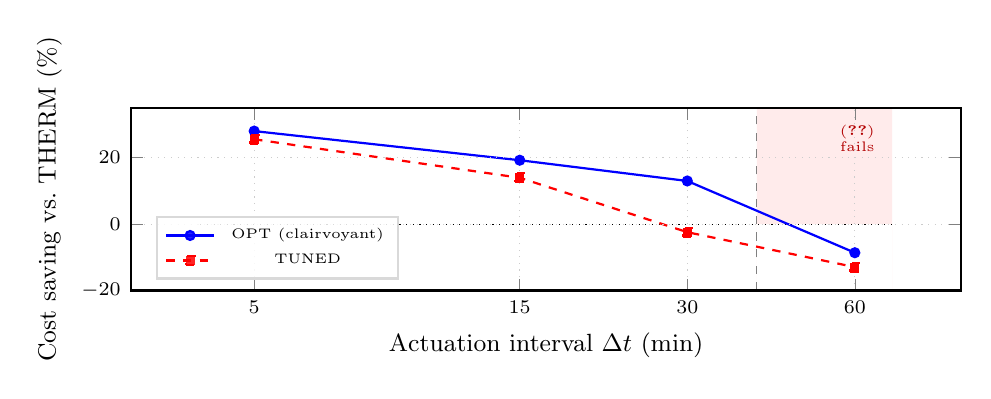
\begin{tikzpicture}
\begin{axis}[
  width=\linewidth, height=3.9cm,
  grid=major, grid style={dotted,gray!40},
  tick label style={font=\scriptsize},
  label style={font=\small},
  legend style={at={(0.5,-0.30)},anchor=north,legend columns=2,
                font=\tiny,draw=gray!30,column sep=4pt},
  thick,
  legend style={at={(0.03,0.06)},anchor=south west,legend columns=1,
                font=\tiny,draw=gray!30,fill=white,fill opacity=0.85,
                text opacity=1},
  xmode=log, log basis x=2,
  xtick={5,15,30,60}, xticklabels={5,15,30,60},
  xlabel={Actuation interval $\Delta t$ (min)},
  ylabel={Cost saving vs.\ THERM (\%)},
  ymin=-20, ymax=35,
  axis on top,
]
\addplot[fill=red!8,draw=none,forget plot]
  coordinates{(40,-20)(40,35)(70,35)(70,-20)}\closedcycle;
\addplot[gray,dashed,thin,forget plot] coordinates{(40,-20)(40,35)};
\addplot[black,dotted,thin,forget plot] coordinates{(4,0)(70,0)};
\addplot[blue,thick,mark=*,mark size=1.6pt]
  coordinates{(5.0,28.03)(15.0,19.25)(30.0,13.0)(60.0,-8.62)};
\addlegendentry{OPT (clairvoyant)}
\addplot[red,thick,dashed,mark=square*,mark size=1.6pt]
  coordinates{(5.0,25.57)(15.0,13.96)(30.0,-2.43)(60.0,-12.95)};
\addlegendentry{TUNED}
\node[font=\tiny,red!70!black,align=center,anchor=north east]
  at (axis cs:68,33) {(\ref{eq:deadband_condition})\\fails};
\end{axis}
\end{tikzpicture}
\caption{Saving vs.\ actuation interval.}
\end{subfigure}\hfill
\begin{subfigure}[b]{0.49\textwidth}
\begin{tikzpicture}
\begin{axis}[
  width=\linewidth, height=3.9cm,
  grid=major, grid style={dotted,gray!40},
  tick label style={font=\scriptsize},
  label style={font=\small},
  legend style={at={(0.5,-0.30)},anchor=north,legend columns=2,
                font=\tiny,draw=gray!30,column sep=4pt},
  thick,
  legend style={at={(0.97,0.94)},anchor=north east,legend columns=1,
                font=\tiny,draw=gray!30,fill=white,fill opacity=0.85,
                text opacity=1},
  xmode=log, log basis x=10,
  xtick={900,1800,4800,9600},
  xticklabels={0.9k,1.8k,4.8k,9.6k},
  xlabel={Thermal capacity $\Cth$ (kJ/K)},
  ylabel={Occupied degree-hours, THERM},
  ymin=-0.3, ymax=3.6,
  axis on top,
]
\addplot[fill=red!8,draw=none,forget plot]
  coordinates{(800,-0.3)(800,3.6)(1800,3.6)(1800,-0.3)}\closedcycle;
\addplot[gray,dashed,thin,forget plot] coordinates{(1800,-0.3)(1800,3.6)};
\addplot[black,thick,mark=triangle*,mark size=2pt]
  coordinates{(900.0,3.0388)(1200.0,2.7371)(1800.0,2.4997)(2400.0,0.0)(4800.0,0.0)(7200.0,0.0)(9600.0,0.0)};
\addlegendentry{THERM comfort leakage}
\addplot[green!55!black,only marks,mark=o,mark size=2.6pt]
  coordinates{(4800,0)};
\addlegendentry{adopted $\Cth$}
\node[font=\tiny,red!70!black,align=center,anchor=south west]
  at (axis cs:845,0.35) {(\ref{eq:deadband_condition})\\fails};
\node[font=\tiny,anchor=west,align=left] at (axis cs:2450,1.35)
  {(\ref{eq:deadband_condition}) holds with \emph{equality}\\at
   $\Cth{=}1800$, yet the baseline\\still leaks $2.50$ degree-hours};
\draw[gray!70,thin,-{Stealth[length=3pt]}]
  (axis cs:2400,1.5) -- (axis cs:1840,2.42);
\end{axis}
\end{tikzpicture}
\caption{Baseline comfort leakage vs.\ capacity.}
\end{subfigure}
\caption{The deadband condition~\eqref{eq:deadband_condition} decides whether a
reported saving is interpretable at all. (a)~Cost saving against the actuation
interval at $\Cth=4800\,$kJ/K: beyond $\Delta t\approx40\,$min the condition
fails and both arms turn negative, because the baseline can no longer hold its
own deadband and the comparison is between two controllers that both violate
comfort. (b)~The baseline's occupied degree-hours against capacity at
$\Delta t=15\,$min. The condition holds with \emph{equality} at
$\Cth=1800\,$kJ/K, and the baseline still leaks $2.50$~degree-hours there: the
condition must hold with margin, not merely hold. Shaded regions mark parameter
choices where~\eqref{eq:deadband_condition} is violated; no saving reported in
them is meaningful. Source: Table~\ref{tab:timestep}.}
\label{fig:admiss}
\end{figure*}
